\documentclass{beamer}
\usepackage[utf8]{inputenc}
\usepackage{amsmath}
\usepackage{ragged2e}

\usetheme{Madrid}
\usecolortheme{default}
\justifying
\usepackage{xcolor}
\definecolor{CorrectGreen}{RGB}{0,100,0} % Dark Green

%------------------------------------------------------------
%This block of code defines the information to appear in the
%Title page
%Information to be included in the title page:
\title[Methodology of Outside Field Dosimetry] %optional
{Methodology of Outside Field Dosimetry}
\subtitle{Acuros as algorithm and Halcyon as a LINAC}


\author[Souvik Das] % (optional)
{
\includegraphics[height=2cm]{Tata_Memorial_Center_logo.jpg} \\ Souvik Das}
\institute[] % (optional)
{
  Resisdent Medical Physicist\\
  Tata Memorial Hospital, Mumbai
}

\date[\today] % (optional)


%End of title page configuration block
%------------------------------------------------------------



%------------------------------------------------------------
%The next block of commands puts the table of contents at the 
%beginning of each section and highlights the current section:

\AtBeginSection[]
{
  \begin{frame}
    \frametitle{Table of Contents}
    \tableofcontents[currentsection]
  \end{frame}
}
%------------------------------------------------------------


\begin{document}

%The next statement creates the title page.
\frame{\titlepage}


%---------------------------------------------------------
%This block of code is for the table of contents after
%the title page
  % \begin{frame}
  % \frametitle{Table of Contents}
  % \setcounter{tocdepth}{2}
  % \tableofcontents[]
  % \end{frame}
%---------------------------------------------------------


%---------------------------------------------------------
% 
%---------------------------------------------------------
\section{Project topic}
\begin{frame}
  \frametitle{Project topic}

  Out of Field Dosimetry in Haclyon using Acuros as algorithm.

  Equipment required: 
  \begin{itemize}
    \item Halcyon LINAC
    \item Eclipse Treatment Planning System
    \item ATOM anthropomorphic male reference phantom (CIRS, Inc., Norfolk, VA)
    \item LD
  \end{itemize}
\end{frame}

\begin{frame}
  \frametitle{Which Site to be investigated?}
  I have to make a dataset which type of patient are lived long after the radiation therpy.
  
\end{frame}


\begin{frame}
  \frametitle{ATOM anthropomorphic male reference phantom}
  \begin{table}
    \centering
    \scriptsize
    \resizebox{\textwidth}{!}{%
      \begin{tabular}{|p{1.8cm}|c|p{2.3cm}|c|c|p{2.1cm}|c|p{2.2cm}|}
        \hline
        \textbf{Description} & \textbf{Model} & \textbf{Available Dosimetry Configurations} &
        \textbf{Height, cm} & \textbf{Weight, kg} & \textbf{Thorax Dimensions, cm} &
        \textbf{Bone Physical Density, cc} & \textbf{Bone Electron Density, 1/cc} \\
        \hline
        Adult Male & 701 & B, C, D \& G & 173 & 73 & 23 cm $\times$ 32 cm & 1.60 &
        $5.030 \times 10^{23}$ \\
        \hline
      \end{tabular}%
    }
  \end{table}

  \vspace{0.15cm}
  \begin{minipage}{\textwidth}
    \tiny
    \textbf{Configuration key:}\quad
    \begin{tabular}{@{}ll@{}}
      B Configuration & = 3 $\times$ 3 cm Grid - 5 mm Holes \\
      C Configuration & = 1.5 $\times$ 1.5 cm Grid - 5 mm Holes \\
      D Configuration & = Organ Grid - 5 mm Holes \\
      G Configuration & = Organ Grid - 14 mm Holes
    \end{tabular}
  \end{minipage}

\end{frame}

\begin{frame}
  \frametitle{ATOM anthropomorphic male reference phantom}
  \framesubtitle{Manufacturer slide}
  \begin{center}
    \includegraphics[page=4,width=\textwidth]{References/ATOMPhantomFamily_031324.pdf}
  \end{center}
\end{frame}


\begin{frame}
  \frametitle{Which Luminescence Dosimeter(LD)?}
  See
\end{frame}








\end{document}

